\documentclass[12pt]{article}
\usepackage{graphicx}
%\usepackage[margin=1in]{geometry}
\usepackage{float}
\usepackage{amsmath}
\usepackage{url}

\restylefloat{figure}
	\title{IT3708 - Exercise 4}
\author{
        Eirik Hammerstad \& Nicklas Utgaard
}

\newcommand{\shiftline}[0]{\hfill\newline\noindent}
\newcommand{\degree}[0]{\ensuremath{^\circ}}

\date{\today}
\begin{document}
\maketitle
\section{Disclaimer}
In order to keep to our tradition of using Java in this course we decided to use it to implement our control system during this project. 
Further is it worth noting that we completed this project with three main iterations, each consisting of several subiterations. 

\shiftline The first iteration was used to implement the general architecture as well as the three submodules, 
	\textit{Search}, \textit{Retrieval}, and \textit{Stagnation}, in a very rudemental way.

\shiftline This formed the basis for our second iteration where we converted most of the provided \textit{C} modules to Java, 
	and introduced \textit{OOP} into these in order to fit into the overall architecture.

\shiftline 	The last iteration of this project was used to identify improvement potential and improve upon these in the three modules implemented during the first iteration. 
The methodology was to look at the behavioural differences between our own implementation and the converted \textit{C} implementation, as well as looking for other 
non progressive behaviour and finding possible mitigations to these.

\section{Part A}
	\subsection{System overview}
		\subsubsection{Architectural description}
			Figure~\ref{fig:architecture} shows the architecture as was at the end of the project. 
			Arrows to packages indicating the usage of all part in that package. 
			E.g \textit{SensoryInput} has an aggregation arrow to the \textit{input} package, which in term indicates that it is an aggregation 
			of the package's internal classes (\textit{LightArray} and \textit{ProximityArray}).
			
			\begin{figure}[H]
				\centering
				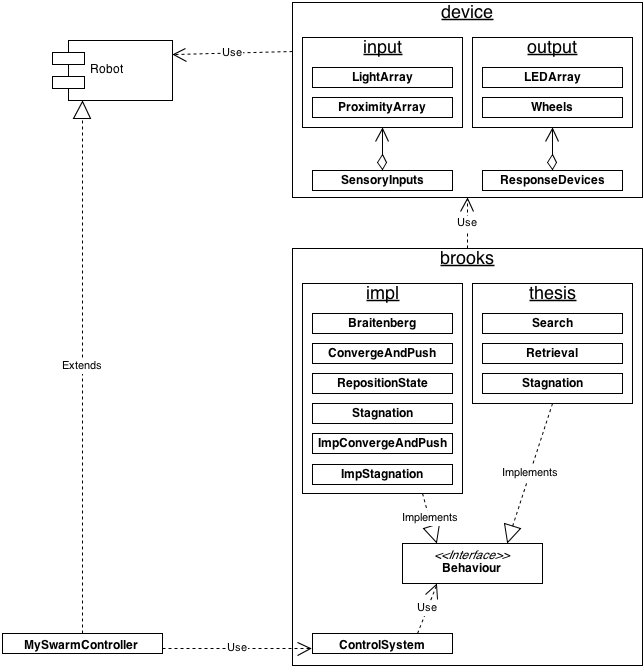
\includegraphics[width=.9\columnwidth]{./../images/brooksArchitecture.png}%
				\caption{Project architecture}
				\label{fig:architecture}	
			\end{figure}
			
			\shiftline In the architecture there are especially four entities worth taking a look at, 
				\textit{MySwarmController}, \textit{ControlSystem}, \textit{Behaviour} and the \textit{device} package.
			
			\shiftline \textit{MySwarmController} is the entrypoint for the controller. 
				It has the responsibility of initating the control system before start, and invoking the \textit{step} method related to webots. 
			
			\shiftline The \textit{ControlSystem} handles initialization of sub modules to be used in the subsumption architecture, 
				and the initialization of the robot abstraction. During runtime it handles invokation of submodules.
			
			\shiftline All behavioural modules implement the \textit{Behaviour} interface. This interface provide two methods, 
				\textit{trigger(SensoryInputs, ResponseDevices):Boolean} and \textit{execute(SensoryInputs, ResponseDevices):Void}. 
				The first method should check if the current world state is perceived in such a way that the module would like to be activated. 
				E.g. the random walk module will always return \textit{True}, since this is the most basic behaviour in our system. 
				The retrieval module on the other hand will check some of the input sensor, and from these make the decision. 
			
			\shiftline The \textit{device} package holds the abstraction entities used to simplify the usage of the robot, 
				and provides aggregated structures of these to minimize the amount of parameters needed to be passed through the architecture. 
				\textit{LightArray}, \textit{ProximityArray} and \textit{LEDArray} provides easy access to the light sensors, distance sensors and all the LED respectively. 
				The one who differentiate itself from the rest is \textit{Wheels}, which is an abstraction layer and extension of the provided \textit{DifferentialWheels}. 
				It was large inspirered by \textit{epuck\_basic.py}.
			
		\subsubsection{Changes to the world}
			The inital settings of the light source caused the epucks to always see the lightsource, additionally the distance to the lightsource seemed
			to have little impact on the sensor readings. Based on this we decided to change the attenuation of the lightsource from $[1,0,0]$ to $[0,0,25]$.
			This gave us the desired behaviour of the lightsource, where the epucks did not detect the source from far away and distance did affect the sensor readings.
			One downside to this change was that in close proximity of the lightsource the sensors would simply yield a zero value for the sensors facing the lightsource.
			We did however dicide to keep this change throughout the project since this effect gave us an more realistic simulation and provided us with more testing possibilities.
			
			%In addition to the "`physical"' change of the world we added a supervisor entity as well. This was done in order to automiaticly run the simulation multiple times
			%without the need to restart manually. The supervisor also provided us with data related to the length of each run and how far the box was pushed.
		
	\subsection{Inital implementation}
		The inital implementation of the control system and behavioural modules focused on getting the control system to work, and just the basics of the modules.
		We used the trinity of modules proposed in the project description, and implemented them in a simple way. 
		
		\shiftline The \textit{Search} module implemented a Braitenberg vehicle, without any means of randomness in the module. 
		
		\shiftline The \textit{Retrieval} module was implemented to phases of retrieval, converge and push. 
			As soon as the sensors picked up light from the lightsensor we aligned the robot such that the front was towards the lightsource and told it to move forwards. 
			Once close enough to the box it shifts for convergance to pushing, in this case it is just trying to keep the forward momentum.
	
		\shiftline The last module implemented was the \textit{StagnationAvoidance}, this module was inspired by the provided \textit{C} code to a large degree, 
		in that we kept realignment and repositioning tasks. 
		We did however use our own implementation of the tasks in order to keep it simple. 
			
		\subsubsection{Performance and issue mitigation}
			The performance of the box varied alot, given enough time they tid eventually get the box to a wall in some cases. But more often then not did some epucks get stuck, 
			either in a corner or against another epuck, and the saw a lot of ``fighting'' (alignment towards epuck instead of box). In some cases these issues were resolved, 
			but we also saw cases were these resulted in complete stagnation of progress. 
			One unexpected feature of our implementation was that it allowed what we came to call "`pushing of pushers"'(see figure~\ref{fig:pushing} p.~\pageref{fig:pushing}), that means that in some cases we saw more then three 
			epucks working together on the same side, which resulted in that it was not enough rom for all of them to get close to the box. In this case the epuck would stand behind
			the three pushing epucks, and push on these instead. 
				

\section{Part B}
	\subsection{Areas of improvement}
		%\subsubsection{Architecture} %If the report size allows for it, add something about building behavioural trees
		\subsubsection{Modules}
			With this inital implementation we identified several issues that needed to be adressed. 
			The \textit{Search} module did in general do what it was supposed to do, we did however find cases where the epucks got stuck in corners. 
			And in some very rare cases would they get stuck pushing against eachother without seeing the other epuck.
		
			\shiftline The \textit{Retrieval} modules did work very well with a small number of epucks. Problem did however arise when to many epucks got close together during
			the pushing phase. The issue came down to alignment with the box, 
			in some cases the epuck lost track of the alignment and instead tried to align itself against its neighbours(see figure~\ref{fig:alignment} p.~\pageref{fig:alignment}). 
			
			\shiftline The \textit{StagnationAvoidance} did work as expected without any major issues. The only problem we were able to find was that trying to turn the
			epuck 90\degree during repositioning would not always be perfect, and hence sending the epuck towards the box with a wrong alignment when it was completed. 
			
			\shiftline In order to migitigate the issues we propose adding randomness to the movement provided by the \textit{Search} module. This will allow the epucks to get 
			unstuck from at least eachother, but also preferably also corners. The \textit{Retrieval} and \textit{StagnationAvoidance} work very close together in the current
			structure, in order to seperate these a bit more we suggest moving the realignment from \textit{StagnationAvoidance} to \textit{Retrieval}, this will give a more 
			clear cut of the responsibilities of each module. It will also change the behaviour of the epucks, such that at all times tries to be aligned with the box
			before starting to push. This "`keep-align"' strategy will avoid the epucks from aligning against eachother. It will also avoid the box being counted as a 
			neighbour when the epuck is nonaligned with the box and looking directly to its sides.
			Based on the "`pushing of pushers"' effect we also suggest making all the backfacing sensors part of neighbours detection, instead of just looking directly
			to the sides. This will promote a higher probability of staying the more help a epuck has.
		
	\subsection{Effect of improvements}
		The randomness in the \textit{Search} was not enough to keep keep epucks from getting stuck in corners, it did however solve the problem with epucks getting stuck with eachother.
		In order to solve the corner problem, we looked at why the epucks did not change direction when approaching a corner. This turned out to be a "`feature"' in braitenberg vehicles, 
		where when a epuck approaches a corner with a 45\degree angle to the two walls its sensors will always keep similar values on the left and right, thus causing the vehicle 
		to keep going straight forward. An if-clause was added to the new implementation to detect and avoid this scenario. 
		
		\shiftline By moving realignment from \textit{StagnationAvoidance} to \textit{Retrieval} we saw a big improvement in how the epucks behaved. 
		They would now keep aligned with box almost always. This also made it possible to make small adjustment often while the epuck kept pushing, 
		instead of stopping the push task to realign. This change also enhanced the "`pushing of pushers"' effect in that it all epucks kept facing in the same direction at all cost. 
		
		
		\shiftline The increase in number of backfacing sensors did however not yield the desired result.
		We experienced no change in the neighbourhood part of the \textit{StagnationAvoidance} and we still
		saw cases where a surrounded epuck would decide to reposition, even though a neighbour count of two or more should prohibit this behaviour. 
		One possible explaination to this could be that epucks do not always make an impact on the distance sensor, or that the sensor has a small
		field of view and therefore does not recognize epucks slightly of center to the sensor.
		
		\shiftline In general we saw an improvement in how fast the epucks was able to move the box from the center to one of the walls. 
		Our inital implementation varied alot in its time usage, sometimes solving the task in about one minute other times using over eight minutes to move the box.
		While our final implementation also was prone to variation it showed in general better performance then the previous implementation. 
		The final implementation had an average time of two minutes to solve the task, which proves a great increase in efficiency compared to the first implementation.
		
\section{Figures}
	More figures can be seen in the zip file delivered. 
	\begin{figure}[H]
		\centering
		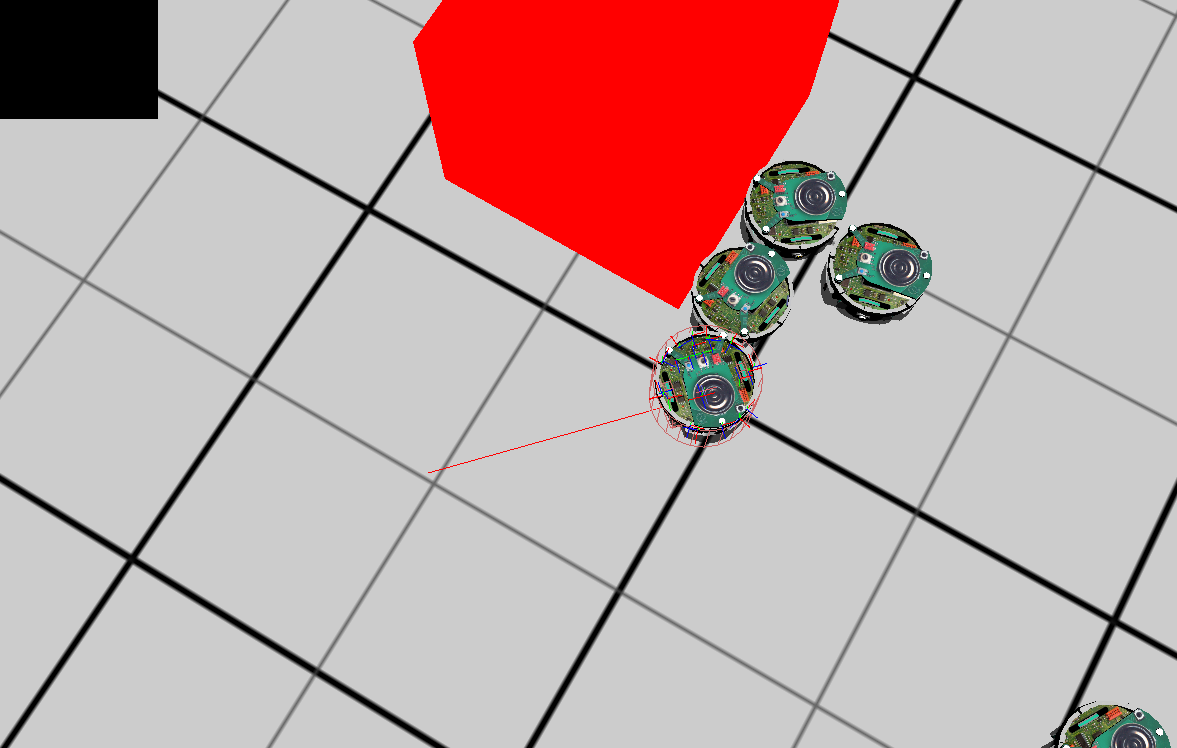
\includegraphics[width=.8\columnwidth]{./images/firstIterationImplementationAlignmentIssue.png}%
		\caption{First iteration alignment issue}
		\label{fig:alignment}	
	\end{figure}
	
	\begin{figure}[H]
		\centering
		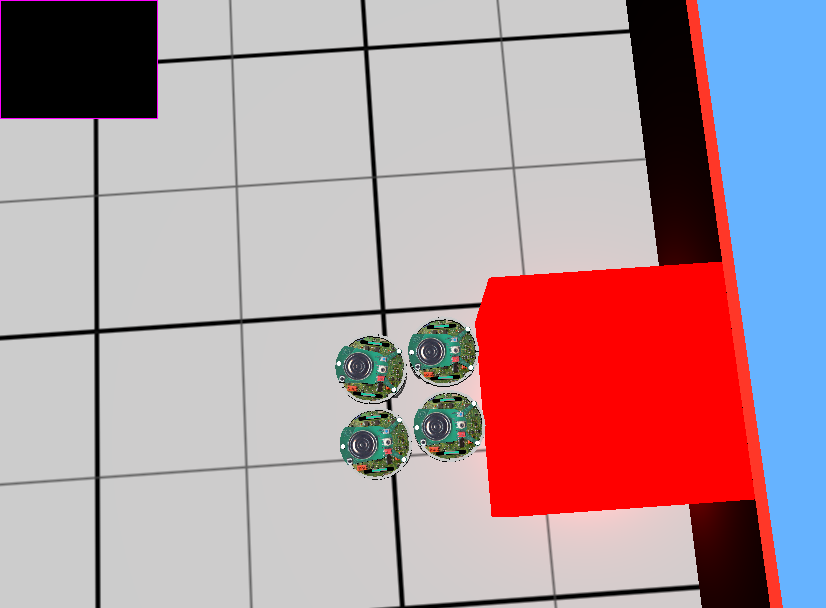
\includegraphics[width=.8\columnwidth]{./images/finalImplementationCompletePushingOfPushers.png}%
		\caption{"`Pushing of pushers"' effect}
		\label{fig:pushing}	
	\end{figure}
\end{document}